\documentclass{article}

\usepackage{xeCJK} 
\usepackage{ijcai13}
\usepackage{amssymb}
\usepackage{amsmath}
\setcounter{tocdepth}{3}
\usepackage{graphicx}
\usepackage{epsfig} 
\usepackage{bm}
\usepackage[usenames]{color}
\usepackage{caption}
\definecolor{lightblue}{rgb}{0, 0, 0}


\bibliographystyle{named}
\setCJKmainfont{WenQuanYi Micro Hei} 
\begin{document}

  
\title{Scalable Graph Hashing with Feature Transformation \\ 
	利用特征变换的可扩展图哈希} 

\author{Qing-Yuan Jiang}
\ead{jiangqy@lamda.nju.edu.cn}
\author{Wu-Jun Li}
\ead{liwujun@nju.edu.cn}

\address{National Key Laboratory for Novel Software Technology }\\
\address{Collaborative Innovation Center of Novel Software Technology and Industrialization}\\
\address{Department of Computer Science and Technology, Nanjing University, China }\\


\maketitle


\begin{摘要}
  
在大数据应用中,哈希因其低存储成本和快速检索速度而被广泛应用于相似邻搜索(ANN)问题。哈希的目标是,将数据点从原始空间映射到二进制码空间,并且保留数据点在原始空间上的相似性(邻域结构)。图哈希是一种备受关注的哈希方法。它直接利用相似性指导哈希码学习。然而,现有的大多数图哈希方法对图形建模的复杂性很高,这使得它们在实际应用中不能取得令人满意的结果。在本文中,我们提出一种新奇的方法,叫做结合特征变换的可扩展图哈希(SGH)。通过特征变换,我们可以有效地近似全图,而不需要计算相似图矩阵。基于此,提出了一种逐位学习哈希函数的连续性学习方法。在两个百万级数据集上的实验表明,我们的SGH方法在准确性和可扩展性方面超越了目前先进的各种哈希方法。

\end{摘要}



%% main text
\section{引言}

最近邻搜索问题\cite{Andoni2010Nearest}在很多领域发挥了重要的作用,比如机器学习、数据挖掘、信息检索等等。在大数据应用中,最近邻搜索的计算通常需要花费很长时间,有时并不能返回查询项的准确最近邻。实际上,近似邻(ANN)\cite{Indyk:1998:ANN:276698.276876,4031381}在很多应用中已经能取得令人满意的表现,比如在搜索引擎上的图像检索问题中。进一步讲,在解决大规模问题时,相似邻搜索通常比最近邻搜索更有效率。因此,在这个大数据时代,相似邻搜索获得了越来越多的关注\cite{4031381}。

因其低存储成本和快速搜索速度,哈希\cite{4031381,Ny2010Semi,PMID:24136430,Zhen:2012:PMM:2339530.2339678,Zhu:2013:LCH:2502081.2502107,Song:2013:IHL:2463676.2465274,Zhang2014SHL,NIPS2014_5332}被广泛用于相似邻搜索问题中。用于ANN搜索的哈希技术通常被称为保相似哈希方法。这种方法将数据点从原始空间投影到汉明空间,同时保存数据点在原始空间上的相似性(邻域结构)。另一方面,海明距离应该尽可能大。哈希方法的时间复杂度是常数级或次线性的\cite{PMID:24136430,Zhang2014SHL}。哈希也能大幅度减少存储空间的使用。举个例子,假设有1百万个数据点,每个点用32位二进制码表示,那么存储这么多数据只需要4GB内存。因此,哈希成为ANN搜索问题的一个有名的解决方案\cite{Gionis:1999:SSH:645925.671516,Datar:2004:LHS:997817.997857,
NIPS2008_3383,Kulis2010Learning,icml2010_WangKC10,
Liu2011Hashing,PMID:24136430,W2012Isotropic,Xu2013Harmonious,Zhang2014SHL,6909650,NIPS2014_5332}。

和传统的数据无关型哈希方法(比如局部敏感哈希(LSH)\cite{Gionis:1999:SSH:645925.671516,Datar:2004:LHS:997817.997857},这种方法不使用数据进行训练)相比,数据相关型哈希方法(也叫做学习型哈希(LH))能使用较短的二进制码取得更好的准确度,这种方法从训练数据中学习哈希函数\cite{PMID:24136430,6247912,Zhang2014SHL,NIPS2014_5332}。因此,LH比数据无关哈希方法更受关注\cite{icml2010_WangKC10,PMID:24136430,6247912,Zhang2014SHL,6909650,NIPS2014_5332}。
现有的学习型哈希方法可以分为两个主要类别\cite{PMID:24136430,6247912,Zhang2014SHL}:无监督哈希和有监督哈希。无监督哈希尝试保留训练数据的欧几里得相似度。有监督哈希\cite{ICML2011Norouzi_246,Zhang2014SHL,6909650}尝试保存带有语义标签的训练数据的语义相似度。虽然有监督哈希在某些应用中表现优异,但是它训练比较耗时。而且,在许多的真实应用中,带标签数据可能难以获取。因此,对于这些应用,我们只能应用无监督哈希进行处理,这也是本文的研究重点。
代表性的无监督哈希方法包括谱哈希(SH)\cite{NIPS2008_3383},二值重构插入(BRE)\cite{Kulis2010Learning},主成分分析哈希(PCAH)\cite{PMID:24136430},迭代量化(ITQ)\cite{PMID:24136430},锚图哈希(AGH)\cite{Liu2011Hashing},各向同性哈希(IsoHash)\cite{W2012Isotropic},离散图哈希(DGH)\cite{NIPS2014_5332}。在这些方法中,SH、BRE、AGH和DGH属于图哈希。直接利用相似性(邻域结构)指导哈希码学习过程,图哈希的优化目标和保相似哈希相一致。因此,在学习算法足够有效的前提下,图哈希应该比其他非图哈希方法表现性能更好。
但是,大多数现有的图哈希方法在实际应用中并不能取得令人满意的表现。这是由于对图形建模复杂度太高。特殊地,相似性通常反映了点对之间的成对关系。存储这种成对关系需要的空间复杂度是$O(n^2)$,其中$n$是训练点的数目。直接计算点对相似度的复杂度也是$O(n^2)$。除了计算和存储相似图的成本之外,几乎所有方法都会在学习过程中产生额外的计算和存储成本。因此,图哈希是耗费空间和时间的一种方法,它从数据集全体中进行学习,这是典型的哈希应用模式。现有的方法必须对大规模数据集进行相似或者采样处理,得到可用于图哈希的数据子集。举个例子,SH假设数据是均匀分布,利用1-D拉普拉斯获得数据集的相似特征函数,这种方法实际上丢失了数据之间的邻域结构。BRE必须从数据集中采样一部分作为训练集,即便存在一个大规模数据集可使用。在实际应用中,SH和BRE都不能取得令人满意的效果,这在已有的实验中已被证明\cite{Liu2011Hashing}。AGH和DGH使用锚图来近似相似图,这使它们的时空复杂度避免达到$O(n^2)$之高。但是,近似的准确度却不能得到保证,这可能会降低学习码的准确度。此外,构建锚图会带来额外的计算成本,在我们的实验中,将会证明这是耗费时间的。总之,虽然图哈希的目标是吸引人的,但在实际应用中,目前现有的方法并不能取得令人满意的结果。
在这篇文章中,我们提出一种新的方法,叫做“利用特征变换的可扩展图哈希(SGH)”,它可用于大规模图像中。SGH的主要贡献如下:

\begin{itemize}
\item  受不对称局部敏感哈希(ALSH)\cite{NIPS2014_5329}的启发,SGH利用特征变换方法来近似整个图,而不是直接计算成对相似图矩阵。因此,SGH的时空复杂度远小于$O(n^2)$,可应用于大规模数据集。
\item 提出了一种连续的学习方法,可以按位学习哈希函数。前比特位造成的残留可以被后比特位捕获。
 \item 在两个百万级数据集上的实验表明,无论是准确度还是可扩展性,SGH都比目前最好的方法效果更好。
\end{itemize}

本文余下的部分组织如下:第二节介绍了本文重点解决的问题,第三节提出了SGH方法。实验在第四节中详细说明,最后,第五节对全文进行了总结。

\section{问题定义}
\subsection{符号}
我们使用黑体小写字母代表向量(如\textbf{v})。\textbf{v}的第$i$的元素表示为$v_i$。黑体大写字母代表矩阵(如 \textbf{V})。\textbf{V}的第$i$行表示为$V_{i*}$,第$j$列表示为$V_{*j}$,第$(i,j)$个元素表示为$V_{ij}$。$V^T$是$V$的转置,$tr(V)$是矩阵$V$的迹。${\|V\|}_F = \sqrt{\sum_{ij}{V_{ij}^2}}$是$F$范数,它可用来定义向量长度。$sgn(\cdot)$是元素级的符号函数。$[u;v]$是两个向量$u$和$v$的连接矩阵。$I_d$是$d$维单位矩阵。

\subsection{图哈希}
假设有$n$个数据点的数据集表示为$X=[x_1;x_2;\ldots;x_n]^T \in R^{n \times d}$,其中,$d$表示数据点的维度,并且$X_{i*}=x^T_i$。不失一般性地,数据被假定为以零为中心,即$\sum_{i=1}^n{x_i=0}$。哈希将每个点$x$映射成一个二进制码$b_i \in \{ -1,+1\}^c$,其中$c$代表码长。总之,我们使用$c$个哈希函数$\{h_k(\cdot)|k=1,2,\cdots,c\}$来计算$x_i$的二进制码,如,$b_i=\[h_1(x_i),h_2(x_i),\cdots,h_c(x_i)\]^T$。

我们有不同的矩阵来度量点对在原始空间上的相似度。令$S_{ij}$表示点$x_i$和点$x_j$之间的相似度。一个广泛使用的标准如下:$S_{ij}=e^{-\frac{{\| x_i-x_j\|}^2_F}{\rho}}$,其中,$\rho >0$是一个参数。我们能发现$S_{ij} \in (0,1]$。哈希需要保存原始特征空间上的相似度。详细地,$x_i$和$x_j$之间的相似度越大,$b_i$和$b_j$之间的汉明距离就越小。换句话说,对三个点$x_i,x_j$和$x_k$,如果$S_{ij} <S_{ik}$,那么$b_k$和$b_i$之间的汉明距离比$b_j$和$b_i$之间的汉明距离小。
如果计算数据集$X$上所有点之间的成对相似度,我们能得到相似图矩阵$S=[S_{ij}]_{n \times n} \in R^{n \times n}$。图哈希尝试使用$\mathbf{S}$的全部或部分信息来学习二进制码。如果我们计算$\mathbf{S}$上全部点的相似度,那么很明显,时空复杂度是$O(n^2)$。这在大规模应用中是不切实际的。因此,如引言中所说,现存的方法必须用近似或采样方法来解决这个问题。但是,它们的性能不能令人满意,这是本文的动机。

\section{利用特征变换的可扩展图哈希}
在这一部分,我们给出图哈希方法SGH的细节,包括模型、学习方法和复杂度分析。

\subsection{模型}
SGH的模型包含两个主要部分:目标函数和特征变换方法。

\textbf{目标函数}}
SGH的目标是通过学习到的哈希码去近似相似矩阵$S$,它的目标函数如下:

\begin{displaymath}
min_{{b_l}^n_{l=1}}\sum^n_{i,j=1}({\tilde{S}_{ij}-\frac{1}{c}b^T_ib_j})^2
\label{eq1}
\end{displaymath}
其中,$\tidle{S}_{ij}=2S_{ij}-1$。注意,$\tidle{S}_{ij} \in (-1,1]$,$S$中的相关距离保存在$\tidle{S}$中。我们在目标函数中使用$\tidle{S}$以和范围$\frac{1}{c}b^T_ib_j \in [-1,1]$保持一致。
直接计算Eq.\ref{eq1}中的二进制码$\{b_l\}$是个NP-hard问题。与核局部敏感哈希(KLSH)\cite{5459466}和核监督哈希(KSH)\cite{6247912}相一致,我们定义$b_i$的第$k$个哈希函数为
\begin{equation*}
h_k(x_i) = sgn(\sum^m_{j=1}{W_{kj}\phi(x_i,x_j)+bias_k})
\end{equation*}
其中,$W \in R^{c \times m}$是权重矩阵,$\phi(x_i,x_j)$是核函数,在我们的实验中,核函数使用RBF(Gaussian)函数。$m$表示核的数目,$bias_k$是偏置项。我们的目标是学习$H(x)=\{h_1(x),\cdots,h_c(x)\}$,来将训练集$\mathbf{X}$映射到二进制矩阵$\mathbf{B} \in \{ -1,+1\}^{n \times c}$,$\mathbf{B}_{i*} = b^T_i$。$bias_k$设置为$-\frac{1}{n}\sum^n_{i=1}\sum^m_{j=1}{W_{kj}\phi(x_i,x_j)}$,这和令训练集在核空间上以零为中心是等效的。实际上,上面的哈希函数可以重写为$h_k(x)=sgn(K(x)w_k)$,其中,$w_k=W^T_{k*}$,$K(x)=[\phi(x,x_1)-\sum^n_{i=1}{{\phi(x_i,x_1)}/{n}},\cdots,\phi(x,x_m)-\sum^n_{i=1}{{\phi(x_i,x_m)}/{n}}]$。然后,将$H(x)$代入Eq.\ref{eq1},我们可以得到包含学习参数$W$的目标函数:
\begin{displaymath}
min_W{{\|c\tilde{S}-sgn(K(X)W^T)sgn(K(X)W^T)^T\|}^2_F}
\label{eq2}
\end{displaymath}
其中,$K(X) \in R^{n\times m}$是$X$上所有训练点的核特征矩阵。
\\

\textbf{特征变换}


正如第二部分所言,如果计算$\tilde{S}$上所有点的成对相似度,它的时空复杂度是$O(n^2)$,这种方法的可扩展性很差。现在,我们提出一种不计算$\tilde{S}$而利用相似度的特征变换方法。
我们首先定义了如下的$P(x)$和$Q(x)$:
\begin{equation}
\begin{split}
P(x)=[\sqrt{\frac{2(e^2-1)}{e\rho}}e^{-\frac{{\|x\|}^2_F}{\rho}}x;\sqrt{\frac{e^2+1}{e}}e^{-\frac{{\|x\|}^2_F}{\rho}};1]\\
Q(x)=[\sqrt{\frac{2(e^2-1)}{e\rho}}e^{-\frac{{\|x\|}^2_F}{\rho}}x;\sqrt{\frac{e^2+1}{e}}e^{-\frac{{\|x\|}^2_F}{\rho}};-1]
\end{split}
\end{equation}
在上面的公式里,我们让$x$乘以一个值$\sqrt{\frac{2(e^2-1)}{e\rho}}e^{-\frac{{\|x\|}^2_F}{\rho}}$,然后加上了两个额外的维度。
接下来我们可以得到
\begin{equation*}
\begin{split}
P(x_i)^TQ(x_j)&=2[\frac{e^2-1}{2e}\times \frac{2x^T_ix_j}{\rho}+\frac{e^2+1}{2e}]\\
&e^{-\frac{{\|x_i\|}^2_F+{\|x_j\|}^2_F}{\rho}}-1\\
&\approx 2e^{\frac{-{\|x_i\|}^2_F-{\|x_j\|}^2_F+2x^T_ix_j}{\rho}}-1\\
&=  2e^{-\frac{-{\|x_i-x_j\|}^2_F}{\rho}}-1\\
&= \tilde{S}_{ij}.
\end{split}
\end{equation*}
这里,我们使用了Figure\ref{fig:one}中的近似关系:当$x\in [-1,1]$时,$\frac{e^2-1}{2e}x+\frac{e^2+1}{2e}\approx e^x$。因此,为了使近似结果合理,我们假设$-1\leq \frac{2}{\rho}x^T_ix_j \geq 1$。这在$\rho = 2\max\rho\{{\|x_i\|}^2_F\}^n_{i=1}$便可得到。实际上,$2\max\rho\{{\|x_i\|}^2_F\}^n_{i=1}$并不是$\rho$的严格约束。在实际应用中,$\rho$被视为超参,我们可用交叉验证技术调整它。
通过这个简单的特征变换,我们派生出了相似度矩阵$\tilde{S} = P(X)^TQ(X)$,其中,$P(X)=\{P(x_1),\cots,P(x_n)\}\in R^{(d+2)\times n}$, $Q(X)=\{Q(x_1),\cots,Q(x_n)\}\in R^{(d+2)\times n}$。如果明确计算$\tilde{S} = P(X)^TQ(X)$,那么时间和空间复杂度依旧是$O(n^2)$。但是,在接下来的学习过程中,我们只使用$P(X)$和$Q(X)$,而不去明确计算$\tilde{S}$。所以,SGH方法的复杂度并不是$O(n^2)$。
请注意,特征变换的思路受启发于ALSH\cite{NIPS2014_5329},该文提出了一种数据无关的最大内积搜索的哈希方法。与ALSH不同的是,SGH属于数据相关型哈希算法。而且,SGH中的特征变换方法与ALSH中的也不相同。

\begin{figure*}[htbp]%位置选项
\centering
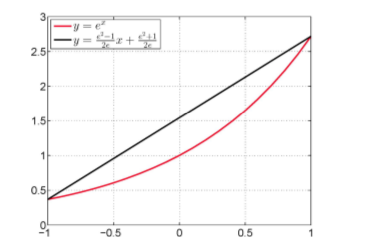
\includegraphics[width=0.5\paperwidth]{figure1.png}
\caption{特征空间上的近似结果}
\label{fig:one}
\end{figure*}

\subsection{学习}
公式\ref{eq2}中的离散$sgn(\cdot)$使得问题变得难以解决。一种可能的解决方案是丢弃离散约束,并将$H(\cdot)$放宽到实值函数上去。SH\cite{NIPS2008_3383}和AGH\cite{Liu2011Hashing}等均采用了这种方案。但是,放松可能会导致性能变差,这已在之前的工作中被证实\cite{W2012Isotropic,Zhang2014Large}。本文中,我们设计了一个逐位的顺序学习策略,前比特位残留的信息将被之后的比特位捕获\cite{6247912,Zhang2014Large}。
假设我们已经学习好了$t-1$个比特。它们对应于权参$\{w_i\}^{t-1}_{i=1}$,剩下的用于计算相似度矩阵的权参计算如下:
\begin{equation}
R_t=c\tilde{S}-\sum^{t-1}_{i=1}{sgn(K(X)w_i)sgn(K(X)w_i)^T}.
\end{equation}
学习第$t$个比特的目标函数如下:
\begin{displaymath}
min_{w_t}{\|R_t-sgn(K(X)w_t)sgn(K(X)w_t)^T\|}^2_F
\label{eq5}
\end{displaymath}
由于存在$sgn(\cdot)$,公式\ref{eq5}中的目标函数依旧是一个NP-hard难题。为了解决这个问题,我们利用谱宽松\cite{NIPS2008_3383}和正交约束得到了以下的式子:
\begin{equation}
min_{w_t}{\|R_t-K(X)w_tw_t^TK(X)^T\|}^2_F\\
s.t. w^T_tK(X)^TK(X)w_t=1
\label{eq6}
\end{equation}

公式\ref{eq6}可进一步简化为:
\begin{equation*}
\begin{split}
&{\|R_t-K(X)w_tw_t^TK(X)^T\|}^2_F\\
 &=tr[(R_t-K(X)w_tw_t^TK(X)^T)(R_t-K(X)w_tw_t^TK(X)^T)^T]\\
 &=tr[K(X)w_tw_t^TK(X)^TK(X)w_tw_t^TK(X)^T]\\
  & -2tr(w^T_tK(X)^TR_tK(X)w_t)+tr(R_tR^T_t)\\
& =-2tr(w^T_tK(X)^TR_tK(X)w_t)+const.
\end{split}
\end{equation*}

之后,公式\ref{eq6}重新被制定如下:
\begin{equation}
\begin{split}
min_{w_t}-tr(w^T_tK(X)^TR_tK(X)w_t)\\
s.t.w^T_tK(X)^TK(X)w_t=1
\label{eq7}
\end{split}
\end{equation}


然后,我们可以得到如下的广义特征值问题:
\begin{equation*}
K(X)^TR_tK(X)w_t= \lambda K(X)^TK(X)w_t.
\end{equation*}

现定义$A_t=K(X)^TR_tK(X)$,则有
\begin{equation*}
\begin{split}
A_t=& A_{t-1}-\\
&K(X)^Tsgn(K(X)w_{t-1})sgn(K(X)w_{t-1})^TK(X)
\end{split}
\end{equation*}
和
\begin{equation}
\begin{split}
A_1=&cK(X)^T\tilde{S}K(X)\\
   =&cK(X)^TP(X)^TQ(X)K(X)\\    
   =&c[K(X)^TP(X)^T][Q(X)K(X)]
\label{eq8}
\end{split}
\end{equation}

公式\ref{eq8}是我们学习算法的重点。从中可以看出,该方法不仅隐式地包含了成对相似度矩阵$\tilde{S}$的全部信息,也成功避开了$O(n^2)$这个高计算和存储成本。
经过从1到$c$的$t$轮迭代,我们能学到矩阵$W=\{w_i\}^c_{i=1}$。实际上,顺序学习过程可以采用下面的残基进一步继续:
\begin{equation*}
R_t=c\tilde{S}-\sum^c_{i=1,i\neq t}sgn(K(X)w_i)sgn(K(X)w_i)^T.
\end{equation*}
我们发现这个过程能进一步提高准确度。在这篇文章中,我们额外进行了$c$轮迭代,前提是保证准确度和速度之间的平衡。
Algotiyhm 1对顺序学习过程进行了简单的总结。实验中,未来避免数值问题,$\gamma$被设置为一个很小的正数:$\gamma =10^{-6}$。

\begin{figure*}[htbp]%位置选项
\centering
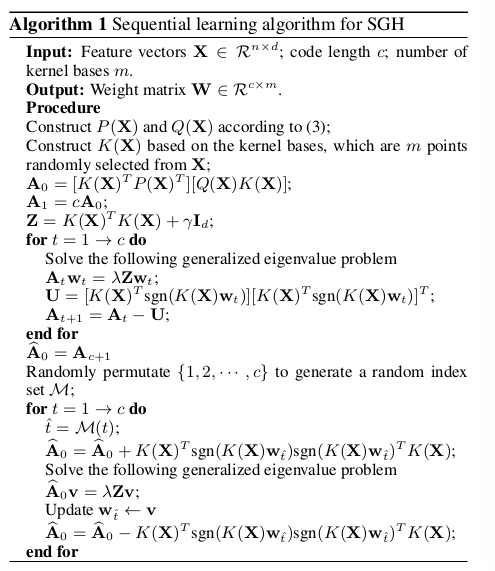
\includegraphics[width=0.5\paperwidth]{alg.png}
\label{fig:alg}
\end{figure*}

% Please add the following required packages to your document preamble:
% \usepackage{multirow}
\begin{table*}
\vspace{-2ex}
\centering

\label{table:one}
\resizebox{\textwidth}{!}{ %
\begin{tabular}{|c|c|c|c|c|c|c|c|c|c|c|}
\hline
\multirow{}{}{Method} & \multicolumn{5}{c|}{TINY-1M}                                                            & \multicolumn{5}{c|}{MIRFLICKR-1M}                                                       \\ \cline{2-11} 
                        & 32bits          & 64bits          & 96bits          & 128bits         & 256bits         & 32bits          & 64bits          & 96bits          & 128bits         & 256bits         \\ \hline
SGH                     & \textbf{0.4697} & \textbf{0.5742} & \textbf{0.6299} & \textbf{0.6737} & \textbf{0.7357} & 0.4919          & \textbf{0.6041} & \textbf{0.6677} & \textbf{0.6985} & \textbf{0.7584} \\ \hline
ITQ                     & 0.4289          & 0.4782          & 0.4947          & 0.4986          & 0.5003          & \textbf{0.5177} & 0.5776          & 0.5999          & 0.6069          & 0.6228          \\ \hline
AGH                     & 0.3973          & 0.4402          & 0.4577          & 0.4654          & 0.4767          & 0.4299          & 0.4741          & 0.4911          & 0.4998          & 0.506           \\ \hline
DGH-I                   & 0.3974          & 0.4536          & 0.4737          & 0.4874          & 0.4969          & 0.4299          & 0.4806          & 0.5001          & 0.5111          & 0.5253          \\ \hline
DGH-R                   & 0.3973          & 0.4554          & 0.4871          & 0.4989          & 0.5276          & 0.4121          & 0.4776          & 0.5054          & 0.5196          & 0.5428          \\ \hline
PCAH                    & 0.2457          & 0.2203          & 0.2000          & 0.1836          & 0.1421          & 0.2720          & 0.2384          & 0.2141          & 0.1950          & 0.1508          \\ \hline
LSH                     & 0.2507          & 0.3575          & 0.4122          & 0.4529          & 0.5212          & 0.2597          & 0.3995          & 0.466           & 0.5160          & 0.6072          \\ \hline
\end{tabular}}
\vspace{-2ex}
\caption{ TINY-1M和MIRFLICKR-1上的Top-1000精确度。最好的准确度已用黑体标出。}
\end{table*}


\begin{table*}[]
\vspace{-2ex}
\centering

\label{table:two}
\resizebox{\textwidth}{!}{ %
\begin{tabular}{|c|c|c|c|c|c|}
\hline
Method & 32bits         & 64bits         & 96bits         & 128bits         & 256bits         \\ \hline
SGH    & 34.59          & 52.37          & 71.53          & 89.65           & 164.23          \\ \hline
ITQ    & 31.72          & 60.62          & 89.01          & 149.18          & 322.06          \\ \hline
AGH    & 18.60+1438.60  & 19.40+1438.60  & 20.08+1438.60  & 22.48+1438.60   & 25.09+1438.60   \\ \hline
DGH-I  & 187.57+1438.60 & 196.99+1438.60 & 518.57+1438.60 & 924.08+1438.60  & 1838.30+1438.60 \\ \hline
DGH-R  & 217.06+1438.60 & 360.18+1438.60 & 615.74+1438.60 & 1089.10+1438.60 & 2300.10+1438.60 \\ \hline
PCAH   & 4.29           & 4.54           & 4.75           & 5.85            & 6.49            \\ \hline
LSH    & 1.68           & 1.77           & 1.84           & 2.55            & 3.76            \\ \hline
\end{tabular}}
\vspace{-2ex}
\caption{TINY-1M上的训练时间(以秒为单位)}
\end{table*}

\begin{figure*}[htbp]%位置选项
\centering
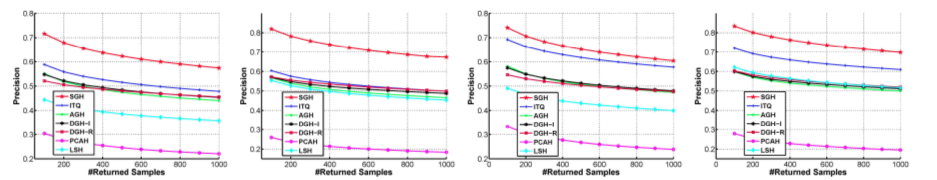
\includegraphics[width=0.6\paperwidth]{figure2.png}
\caption{TINY-1M 和 MIRFLICKR-1M的Top-K精确度}
\label{fig:two}
\end{figure*}


\begin{figure*}[htbp]%位置选项
\centering
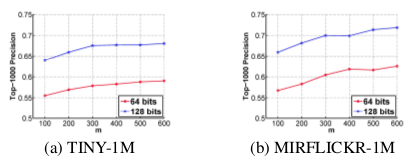
\includegraphics[width=0.6\paperwidth]{figure3.png}
\caption{不同核数目下的Top-1000精确度}
\label{fig:three}
\end{figure*}

\begin{table*}[]
\vspace{-2ex}
\centering

\label{table:three}
\resizebox{\textwidth}{!}{ %
\begin{tabular}{|c|c|c|c|c|c|}
\hline
Method & 32bits         & 64bits         & 96bits         & 128bits        & 256bits         \\ \hline
SGH    & 41.51          & 59.02          & 74.86          & 97.25          & 168.35          \\ \hline
ITQ    & 36.17          & 64.61          & 89.50          & 132.71         & 285.10          \\ \hline
AGH    & 17.99+1564.86  & 18.80+1564.86  & 20.30+1564.86  & 19.87+1564.86  & 21.60+1564.86   \\ \hline
DGH-I  & 85.81+1564.86  & 143.68+1564.86 & 215.41+1564.86 & 352.73+1564.86 & 739.56+1564.86  \\ \hline
DGH-R  & 116.25+1564.86 & 206.24+1564.86 & 308.32+1564.86 & 517.97+1564.86 & 1199.44+1564.86 \\ \hline
PCAH   & 7.65           & 7.90           & 8.47           & 9.23           & 10.42           \\ \hline
LSH    & 2.44           & 2.43           & 2.71           & 3.38           & 4.21            \\ \hline
\end{tabular}}
\caption{MIRFLICKR-1M上的训练时间(以秒为单位)}
\vspace{-2ex}
\end{table*}

\begin{figure*}[htbp]%位置选项
\centering
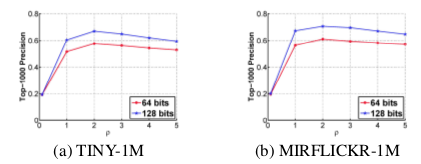
\includegraphics[width=0.6\paperwidth]{figure4.png}
\caption{不同\rho取值下的Top-1000精确度}
\label{fig:four}
\end{figure*}



\subsection{复杂度分析}
计算成本包含两个部分:初始化和主要过程。初始化的复杂度是$O(dn+dmn+mn+(m^2+mn)(d+2)+m^2n)$,包括初始化$P(X)$、$Q(X)$,核初始化,$A_0$和$\mathbf{Z}$的初始化。主要过程的复杂度是$O(c(mn+m^2)+m^3)$。通常说来,$m,d,c$远小于$n$。因此,即便使用了$n^2$个相似项,SGH的时间复杂度也只是$O(n)$。此外,由于没有明确计算相似矩阵$\tilde{S}$,SGH的空间复杂度也是$O(n)$。总之,SGH不仅能获得较高的准确度,并且也具有可扩展性。



\section{实验}
我们在两个百万级数据集上对SGH进行评价。所有的实验在一台Intel (R) CPU E5-2620V2@2.1G、12核、64G RAM的机器上开展。


\subsection{数据集}
我们在两个广泛使用的大规模数据集上评价我们的方法:\emph{TINY-1M}\cite{NIPS2014_5332}和\emph{MIRFLICKR-1M}\cite{Huiskes2010New}。
第一个数据集\emph{TINY-1M}包含一百万张图片。图片原始大小为$32\times 32$。使用GIST特征描述符,每一张微图片用一个384维的特征向量表示。
第二个数据集\emph{MIRFLICKR-1M}来自于莱顿大学LIACS媒体实验室。里面包含从Flickr上爬下来的一百万张图片。我们从每个图片上行提取512维的特征向量。


\subsection{评估指标和基线}
在每个数据集上,我们随机选取5000个数据作为测试集,剩下的作为训练集。与查询项的欧氏距离在头2\%d的数据作为查询项的真实邻居。所以每个查询项有19900个真实邻居。
作为对比的基线方法包括一个数据无关哈希LSH\cite{Datar:2004:LHS:997817.997857},2个典型的无监督哈希AGH\cite{Liu2011Hashing}和DGH\cite{NIPS2014_5332},2个线性投影方法PCAH\cite{PMID:24136430}和ITQ\cite{PMID:24136430}。由于初始方法的不同,DGH产生两个变体\cite{NIPS2014_5332},DGH-I和DGH-R,这两个方法都用作实验基线。留意到SH和BRE这两个图哈希方法并没有在实验中用到,这是因为先前的工作已经证明AGH和DGH的表现优于这两种图哈希方法\cite{NIPS2014_5332}。在构建核特征时,我们采用高斯函数作为核函数,并且随机采样了300个数据点作为核。在$P(X)$和$Q(X)$中,我们设置$\phi =2$。基线方法的设置均与原作者的实验保持一致。
Top-K精确度\cite{NIPS2014_5332}被用来评价我们的方法和基线。在实际应用中,如搜索引擎,用户可能只对查询项顶部的返回结果感兴趣。因此,Top-K精确度可作为一个好的评价指标。



\subsection{准确度}
表\ref{table:one}给出了基于海明排序的Top-1000精确度。我们可以发现SGH几乎在所有情况下准确度都是最高的(MIRFLICKR-1M,32bits情况除外)。特别地,在所有情况下,SGH的性能高于其它图哈希方法。这表明SGH能够有效捕捉数据中的相似信息。
图\ref{fig:two}描述的是64位和128位编码下,不同K取值在两个数据集上的Top-K精确度。比特位设为其它数值时,结果与图\ref{fig:two}相似,为了节省空间,此处将之删去。我们可以看到SGH在不同的K值下准确度最高。





\subsection{速度}
我们在表\ref{table:two}和\ref{table:three}中分别记录了在2个数据集上耗费的时间。请注意“+1438.60”和“+1564.86”表示AGH和DGH构建锚图所花费的时间。将这部分时间加入比较是公平的,因为我们的SGH方法也包含了所有训练时间。从表中可得,SGH在所有情况下都快于AGH和DGH,在大多数情况下快于ITQ。虽然LSH和PCAH比SGH快,但它们的准确度只是差强人意。


\subsection{参数敏感性}
图\ref{fig:three}描述的是不同取值的核数目下,SGH在2个数据集上的Top-1000精确度。从中能够看出,m越大时,准确度越高。但是,m取值较大时会导致计算成本的增加。因此,在实际应用中,我们需要选择合适的m值以平衡准确度和计算成本。
图\ref{fig:four}描述的是不同取值的$\rho$下,SGH在2个数据集上的Top-1000精确度。可以发现,当$1 \leq \rho \geq 5$,准确度变化并不大。实验中,我们令$\rho =2$取得了相对最好的准确度。

\section{总结}
在这篇文章中,我们提出了一个新奇的用于大规模图哈希的方法,叫做SGH。通过避免明确计算相似度矩阵,SGH保证了自身的可扩展性。同时SGH保留数据集中的全部相似信息。实验表明,SGH在准确性和可扩展性方面超越了目前最先进的方法。

\section{致谢}
这项工作得到了国家自然科学基金(编号61472182)和中央高校基本科研基金(20620140510号)的支持。

\bibliography{sghref}


\end{document}

